\documentclass[runningheads]{llncs}

%% Language and font encodings
%\usepackage[english]{babel}
%\usepackage[utf8x]{inputenc}
%usepackage[T1]{fontenc}

%% Sets page size and margins
\usepackage[a4paper,top=3cm,bottom=2cm,left=3cm,right=3cm,marginparwidth=1.75cm]{geometry}

%% Useful packages
\usepackage{amsmath}
\usepackage{graphicx}
\usepackage[colorinlistoftodos]{todonotes}
\usepackage[colorlinks=true, allcolors=blue]{hyperref}
\usepackage{bmpsize}
%\usepackage{subfig}
\usepackage{subcaption}

\newtheorem{define}{Definition}
\newtheorem{thm}{Theorem}
\newtheorem{axiom}{Axiom}
%\newtheorem{lemma}{Lemma}
%\newtheorem{cor}{Corollary}

\newcommand{\cks}[1]{\textcolor{red}{cks: #1}}
\newcommand{\ab}[1]{\textcolor{cyan}{ab: #1}}

%% Paper specific commands
%Concrete
\newcommand{\texttrue}{\ensuremath{\mathtt{\textsc{true}}}}
\newcommand{\textfalse}{\ensuremath{\mathtt{\textsc{false}}}}

\newcommand{\hardwaredesign}{\ensuremath{P}}
\newcommand{\concstates}{\ensuremath{C}}
\newcommand{\concstate}{\ensuremath{c}}
\newcommand{\concexecution}{\ensuremath{\mathrm{concEx}}}
\newcommand{\concinputs}{\ensuremath{I}}
\newcommand{\concinput}{\ensuremath{i}}
\newcommand{\inputvariable}{\ensuremath{i}}
\newcommand{\variable}{\ensuremath{v}}
\newcommand{\variables}{\ensuremath{V}}
\newcommand{\concvalue}{\ensuremath{x}}
\newcommand{\concexpression}{\ensuremath{e}}
%Symbolic
\newcommand{\symbolicexecutionengine}{\ensuremath{M}}
\newcommand{\symstates}{\ensuremath{S}}
\newcommand{\rootsymstate}{\ensuremath{s_0}}
\newcommand{\symstate}{\ensuremath{s}}
\newcommand{\symvalue}{\ensuremath{\sigma}}
\newcommand{\syminputs}{SymInputs}
\newcommand{\syminput}{\ensuremath{\alpha}}
\newcommand{\symexecution}{\ensuremath{\mathrm{symEx}}}
\newcommand{\pathconditions}{\ensuremath{\mathit{PC}}}
\newcommand{\pathcondition}{\ensuremath{\mathit{pc}}}
\newcommand{\symalphabet}{\ensuremath{\Sigma}}
\newcommand{\trees}{\ensuremath{T}}
\newcommand{\tree}{\ensuremath{t}}
\newcommand{\nodes}{\ensuremath{N}}
\newcommand{\symexpression}{\ensuremath{\sigma}}


\begin{document}

\title{A Recursive Strategy for Symbolic Execution Expressed in Coq}
\author{A. Byrnes and C. Sturton}

%%\authorrunning{F. Author et al.}

\institute{University of North Carolina at Chapel Hill Department of Computer Science, \\  201 S Columbia St, Chapel Hill, NC 27599 \\
\email{\{abyrnes1,csturton\}@cs.unc.edu}}


\maketitle

\begin{abstract}
Prior work has proposed the use of symbolic execution for the security
validation of a processor design. The approach uses a recursive search strategy
that is designed to counter the exponential path growth inherent in multi-cycle
processor execution. In this work, we examine the search strategy in order to
prove its correctness. We formulate an abstract model of symbolic execution with
the recursive search strategy in Coq, and we find that the
strategy as proposed is not guaranteed to be sound---that is, the
search may find a symbolic path for which no concrete path from the processor's initial state
to the given error state exists. We tighten one of the requirements of the
search strategy and then prove the modified strategy correct. 
\end{abstract}

\section{Introduction}
%\cks{15 pages, excl. bib, excl. appdx}

Researchers have recently begun exploring the use of software-style symbolic execution for the
verification of hardware designs~\cite{mukherjee2015hardware,liu2009star}. Symbolic execution has a proven track record in the software community as a
bug-finding tool~\cite{cadar08,cha12,do16} and as an aid in formal
verification~\cite{chi16,davidson13}. However, bringing these benefits to bear on hardware
designs has been a challenge---the complexity of the search space of relatively
simple hardware designs more closely resembles that of large, continuously interactive
software systems than that of the stand-alone software programs that are the classic
targets of symbolic execution. In response to this challenge a recent paper proposed a recursive
search strategy for symbolic execution~\cite{zhang2018recursive}. Zhang et
al.~showed the strategy to be
practical~\cite{zhang2018end}, but the soundness of the approach has not been
demonstrated. A proof of correctness is needed.

In this paper we prove that a recursive search strategy for the
symbolic execution of hardware designs is sound: a list of
constraints returned by a successful search defines a set of concrete input
sequences, each of which will take the processor from its initial reset state to
an error state.

Our goal is to validate the search strategy itself rather than any one implementation
of it. Therefore we decouple our model of symbolic execution from the particular
programming language to be symbolically executed. We formalize an abstract model of symbolic
execution in Gallina, the specification language of the Coq proof
assistant~\cite{coqreference}; the structure of the model is built
around the three fundamental properties of symbolic execution as first laid out
by King in 1976~\cite{king1976symbolic}. This has the advantage of providing soundness
guarantees for the recursive search strategy when implemented by any symbolic
execution engine which abides by the three King properties.

The symbolic exploration of a program produces a rooted, binary tree. The root
node represents the entry point of the program, and each path from root to a
leaf node represents one possible path of the execution through the program.
Although the mechanics are similar, the symbolic exploration of a hardware
design differs from this model conceptually: The tree produced by the symbolic exploration of a
hardware design represents the state transitions possible in a single clock
cycle from a given state (the root node). A sequence of state transitions, for
example from the hardware's initial, reset state to an error state is
represented by a sequence of trees. The set of all possible $n$ transitions from
a given state requires a tree (of depth $n$) of trees.

The strategy proposed by Zhang and Sturton tackles this search complexity with a
recursive search. First the $n^{\mathrm{th}}$ tree in the desired sequence of
trees is found, then the $n-1^{\mathrm{st}}$ tree, and so on, until the first
tree in the sequence, whose root node starts at the reset state, is
found.\footnote{The problem is undecidable in the general case, and Zhang et
  al. introduce a set of heuristics to make it work in
  practice~\cite{zhang2018end}.} The strategy lays out three properties that, if
satisfied at each iteration of the search, are sufficient to ensure the final
sequence of paths through trees represents a possible, multi-cycle sequence of
state transitions from the hardware's initial state to the desired (error)
state.

The bulk of our proof is a proof by induction over the sequence of trees to show
that the trees are correctly stitched together. In the base case we show that
symbolic
execution, as defined by King, implies the correct \emph{concretization} of a path through a
single symbolic execution tree as defined by Zhang and Sturton. In the inductive
step we show that a path through a sequence of trees stitched together according
to the Zhang and Sturton requirements will yield a correct concretization of a
path through the sequence of trees. Finally, we prove that the sequence begins in a reset state and ends in the
desired error state.

We find that the recursive search strategy as originally proposed is not sound---that is, the
search may find a symbolic path for which no concrete path from the processor's initial state
to the given error state exists. We tighten one of the three
requirements of the strategy and then prove the modified strategy is sound.

We present two contributions of this work:
\begin{itemize}
  \item An abstract model of symbolic execution expressed in the Coq
    framework. This model can form the starting point for 
    building a provably correct implementation of a symbolic execution engine for a
    particular language. We make our model available online.
\item We verify the soundness of the recursive search strategy for symbolic
  execution. We find and fix a flaw in the original formulation of the
  strategy. The recursive search strategy was originally developed for
  the verification of hardware designs; however, any symbolic execution engine that
  implements the proven strategy will be assured the same guarantee of soundness.
\end{itemize}

\section{Prior Work}
Symbolic execution was first formally defined by King in 1976~\cite{king1976symbolic} and has
been widely adopted by the software engineering and software security
communities. (See Schwartz et al.~\cite{schwartz2010all} for a recent survey.)

Symbolic execution has since shown practical value through implementations. Anand et al. introduced a tool JPF-SE that works as an extension of the Java PathFinder model checker to allow for symbolic execution of Java programs~\cite{anand2007jpf}.  P{\u{a}}s{\u{a}}reanu et al. later introduced the tool Symbolic PathFinder that also utilizes Java Path Finder to symbolically execute Java bytecode~\cite{puasuareanu2010symbolic}. Noller et al. recently released a tool that utilizes Java PathFinder to perform ``shadow symbolic execution'' on Java bytecode~\cite{Noller2018}.

\subsection{Use of Symbolic Execution in Hardware}
In addition to the paper by Zhang and Sturton that lays out the three-part
strategy we prove here~\cite{zhang2018recursive}, there are a handful of papers that examine
the use of symbolic execution in hardware. In a subsequent paper, Zhang et
al.~\cite{zhang2018recursive} make use of their recursive strategy to find new security
vulnerabilities in processor designs. Their work demonstrates that the strategy
is useful in practice.

Prior work first explored the use of software-style symbolic execution for hardware designs. The STAR tool combines symbolic and concrete simulation of hardware designs to
provide high statement and branch coverage~\cite{liu2009star}; PATH-SYMEX uses
forward symbolic execution applied to an ANSI-C model of the hardware
design~\cite{mukherjee2015hardware}. Both tools use a forward search strategy
and have limits on how deep or broadly they can search.

\subsection{Formalization of Symbolic Execution}

Some work has been done to formalize symbolic execution. 
Arusoaie et al. provide a formal framework for a symbolic execution tool that is language-independent~\cite{arusoaie2014generic,arusoaie2015symbolic,lucanu2017generic}. 
However, they don't provide a formal representation of King's branching properties~\cite{king1976symbolic} nor do they formally verify their tool or its outputs. 

\subsection{Backward Search Strategies in Symbolic Execution}

A backward search strategy for symbolic execution of software has been
studied~\cite{ma2011directed,chandra09,dinges04,charreteur10}. Although, to
  the best of our knowledge, the
  requirements for soundness have not been examined in the literature. 
  There the approach is to search
backward through function call chains from a goal line of code to the program's
entry point. The strategy is hindered by complications that arise in software,
such as floating point calculations and external method calls. To the best of our knowledge, the strategy has not been formalized
in the software community, nor its validity proven.


\section{Background}
\cks{SE w/formalization; statement of King properties; SE for HW; explanation of
  RecSE; statement of 3 RecSE properties}
Symbolic execution is a means of exploring many paths through a program
in order to find paths leading to an error state or bug. In symbolic execution
input variables to a program are given symbolic values. As the program executes
the symbolic values are used in place of the usual concrete literals and the
resulting symbolic expressions may propagate throughout the program's
state. Figure~\ref{fig:se} demonstrates the idea. For example, for the code in
Figure~\ref{fig:sea}, if $\mathtt{reset}$ and $\mathtt{count}$ are initialized
with the symbolic values $r_0$ and $c_0$, respectively, then after symbolically
executing lines 1, 3, and 4 count may be set to the symbolic expression $c_0 +
1$ as shown in Figure~\ref{fig:sec}. In addition to the (partially) symbolic
state that is maintained, a symbolic execution engine keeps track of the
\emph{path condition}. The path condition is a conjunction of propositions that
accrue at each conditional branch point in the program. There is one path
condition per path of execution through the code. In Figure~\ref{fig:sec} the
path condition for the path through lines 1, 3, 4, 5, 6 is shown. When execution
reaches the $\mathtt{ERROR}$ at line 6 the path condition is $\mathit{pc} := r_0
== 0 \wedge c_0 + 1 > 3$. This expression can then be solved using a standard,
off-the-shelf SMT solver to find a satisfying solution, say $r_0 := 0$ and $c_0
:= 3$. Substituting these values for $\mathtt{reset}$ and $\mathtt{count}$,
respectively and executing the code concretely could cause execution to follow
the same path as was followed symbolically.

More formally, ...



\section{Definitions and Notation}
\subsection{Processor Model}
\label{sec:procmodel}
In the formalization of their search strategy~\cite{fmspaper}, Zhang et
al. model a processor as a tuple $M = (S, s_0, I, \delta, O, \omega)$, where
\begin{itemize}
  \item $S = \{s_0, s_1, \ldots, s_k\}$ is the finite set of states of the
    processor,
  \item $s_0 \in S$ is the initial state of the processor,
  \item $I = \{0,1\}^n$ is the finite set of input strings to the processor,
  \item $\delta: S \times I \rightarrow S$ is the transition function of the processor,
  \item $O = \{0,1\}^m$ is the finite set of output strings of the processor,
    and
  \item $\omega: S \rightarrow O$ is the output function of the processor.
\end{itemize}

A state $s \in S$ is determined by the values of the \emph{stateful} registers
of the design. These include both architectural registers, which are visible to
software, and microarchitectural registers, which are not visible to
software. Examples of the former include general purpose registers, the stack
pointer, the instruction pointer, and some control registers. Examples of the
latter include the buffers between stages of a pipeline, branch prediction
registers, reorder buffers, and many control signals. They are stateful in that
they hold their current value up to and until getting updated at the next clock
cycle. As such, their current value can be an input to the calculation of their
next-state value. 

The initial state $s_0$ represents the starting state of the processor after a
power-on or reset cycle. Many registers have a value of 0 in this state.

An input string $i \in I$ represents the concatenation of the several input
signals to the processor. The string has a fixed length $n$. The list of input
signals includes the instructions and data fetched from memory (or from a
cache), plus control, error, debug, and interrupt signals.

The transition function $\delta$ defines how state is updated in a single clock
cycle. It is left-total: for every $s \in S$ and every $i \in I$, $\delta$ is defined.

An output string $o \in O$ represents the concatenation of the several output
signals of the processor. The string has a fixed length. The list of output
signals includes addresses and data values to be written to memory, control
signals, and error signals.

The output function $\omega$ determines the value of $o$ in each clock cycle. It
is typically the identity function taken over a subset of the stateful registers
in the design.

\subsection{Coq Model of a Processor Design}
\cks{Come back to this}
We represent a register transfer level hardware design as a tuple $\hardwaredesign =
(\registers,\inputsignals,\assignments_{\registers},\assignments_{\inputsignals},\init,\delta)$, which is defined as
follows.
\begin{itemize}
\item $\registers = \{r_0,r_1,\ldots,r_n\}$ is the finite set of state-holding
  registers in the design.
\item $\inputsignals = \{\inputsignal_0, \inputsignal_1, \ldots,
  \inputsignal_m\}$ is the finite set of input signals to the design.
\item $\assignments_{\registers} \subseteq \{0,1\}^d$
  is the finite set of assignments---valuations---to the state-holding registers. An assignment $\assignment \in \assignments_{\registers}$ is a bitvector that is the
  concatenation of valuations to all registers in $\registers$.
\item $\assignments_{\inputsignals} \subseteq \{0,1\}^e$ is the finite set of
  assignments---valuations---to the input signals. An assignment $\assignment
  \in \assignments_{\inputsignals}$ is a bitvector that is the concatenation of
  valuations to all input signals in $\inputsignals$.
\item $\init \in \assignments_{\registers}$ is the valuation to state-holding
  registers immediately after the hardware design's initialization sequence
  completes. $\init$ represents the initial state of the hardware
  design.
\item $\delta: \assignments_{\registers} \times
  \assignments_{\inputsignals} \rightarrow \assignments_{\registers}$ is the
  transition function, which represents execution of the hardware
  design. 
\end{itemize}

The set $\registers$ are the stateful registers of the design. These are exactly
the set of registers that make up the state $s \in S$ in the abstract tuple
described in Section~\ref{sec:procmodel}.

A valuation $\assignment \in \assignments_{\registers}$ represents a concrete
state of the design. The length $d$ of the valuation bitvector is fixed for a
given design; every state is represented by a bitvector of length $d$. We do not
require, however, that all registers $r_i, r_j \in \registers$ have the same bit
length. the size of the state space of the design is determined by $d$:
$|\hardwaredesign| = 2^d$.

The initial state of the design, $\init$, is sometimes called the reset state and is the
valuation of the state-holding registers immediately after the power-on
cycle completes.

The transition function, $\delta$, is left-total: for every
$\assignment_{\registers} \in \assignments_{\registers}$ and every
$\assignment_{\inputsignals} \in \assignments_{\inputsignals}$, $\delta$ is
defined.

We do not model the output of the
module explicitly; it is the identity function taken over a subset of the
state-holding registers in the design.

%% \cks{scrap: to a
%%   bitvector of length $d$. The bitvector represents the concatenation of valuations to registers $r_0,
%%   r_1, \ldots, r_n$ and inputs signals $\inputsignal_0, \inputsignal_1, \ldots,
%%   \inputsignal_m$. The length of the bitvector, $d$, can be thought of in some
%%   sense as the length or dimension of hte design.   We use $\assignment_{\registers}$ or $\assignment_{\inputsignals}$ to refer to the
%%   slice of an assignment that pertains to the valuation of just the state
%%   holding registers or just the input signals, respectively.
%%  }
%%   $\inputsignals$. It is useful to treat each $\assignment \in \assignments$ as
%%   a tuple $(\assignment_{\registers},\assignment_{\inputsignals})$ in which
%%   $\assignment_{\registers} = \assignment[0:c]$ is the bitvector valuation to
%%   only the state-holding registers and $\assignment_{\inputsignals} =
%%   \assignment[c:d]$ is the bitvector valuation to only the input
%%   signals.\footnote{In this slice notation the first index is inclusive
%%     and the second index is exclusive.} Let $\assignments_{\registers}$ be the
%%   set of all $\assignment_{\registers}$ and $\assignments_{\inputsignals}$ be
%%   the set of all $\assignment_{\inputsignals}$.

%% A state $\concstate \in \concstates$ of the module is a concrete valuation to all
%% registers in the design: $r_0 = i, r_1 = j, \ldots, r_m = k$, where $r_0, r_1,
%% r_m$ represent the stateful registers and $i, j, k
%% \in \{0,1\}^*$. 
%% The domain of the module is the set of binary strings of length $n$, which
%% represents the concatenation of multiple input parameters to the module.
%% The transition function takes the module from one state to the next state. It
%% represents the execution of a single clock-cycle in hardware. 

\subsection{Symbolic Execution}
\cks{*********HERE************}

The result of symbolic execution is a rooted, binary tree $\tree = (N, E, l)$, where
$N$ is the set of nodes of the tree, $E$ is the set of directed edges connecting
two nodes, and $l \in N$ is a particular leaf node of interest in the tree. This
leaf node represents a desired next-state of the module being symbolically
explored, and in the recursive strategy, it is this leaf node that is joined to
the root node of a subsequent tree in the search.

Each node $n \in N$ of the tree is a tuple $n = (\symstate, \pathcondition)$, where
\begin{itemize}
\item $\symstate$ is a (partially) symbolic state of the module and
\item $\pathcondition$ is the current path condition.
\end{itemize}

A symbolic state assigns a symbolic expression, \symexpression, to every register in the design: $r_0 =
\symexpression_0, r_1 = \sigma_1, \ldots, r_m = \sigma_m$. A symbolic expression
\symexpression{} contains at least one symbol and may contain zero or more concrete
literals, arithmetic operators, and logical operators. Examples of
symbolic expressions include `$\alpha$' and `$\alpha + 1$,' where
$\alpha$ is a symbol used by the symbolic execution engine.

A path condition, \pathcondition, is a conjunction of propositions involving
symbolic expressions. For example `$\pathcondition = \alpha + 1 \ge 0 \wedge \alpha < 1$' is a
possible path condition.

We define \symexecution() for a particular hardware module as an abstract method
that takes as input an initial symbolic
state $\symstate$, an initial path condition $\pathcondition_0 = \texttrue$, and a
set of symbolic inputs, and 
returns a tree of explored paths. In the recursive strategy, \symexecution{} is
always called with an initial
symbolic state that is fully symbolic: $r_0 = \alpha, r_1 = \beta, \ldots, r_m = \omega$.

The alphabet of symbols that can appear in a path condition is the union of the
alphabet of symbols used to define a symbolic state and the alphabet of symbols
used as input values by \symexecution{}: $\Sigma_{\pathcondition} = \Sigma_{\symstate} \cup \Sigma_i$.

\subsection{Coq Model of Symbolic Execution}
    \cks{ToDo}
    

%% We model a symbolic execution engine as a tuple $\symbolicexecutionengine =
%% (\symstates, \rootsymstate, \symalphabet, \pathconditions, \symexecution,  
%% \trees)$, where
%% \begin{itemize}
%% \item $\symstates$ is the set of (partially) symbolic states : $\{(\variable_0,\symvalue), (\variable_1,\symvalue), \ldots, (\variable_n,\symvalue)\}$
%% \item $\rootsymstate \in \symstates$
%% \item $\symexecution: \{\symstates,\pathcondition\}
%%   \times \{\syminputs\} \rightarrow \trees$
%% \item $\pathconditions$
%% \item $\symalphabet$ The alphabet of symbols that appear in symbolic expressions
%%   and symbolic assignments.
%% \item $\trees$ The set of trees $\tree = \{E,\nodes\}$. Each tree is a binary tree of nodes.
%% \end{itemize}


%% \begin{itemize}
%% \item $\pathcondition \in \pathconditions$ is the path condition of a particular node of a tree.
%% \item $\pathconditions \subseteq \mathrm{symexpressions}$ Path condition is a subtype of
%%   symexpressions. The set of all path conditions is a subset of the set of all
%%   symexpressions.
%% \item $\nodes: \{\symstate,\pathcondition\}$, where $\symstate \in \symstates$
%%   and $\pathcondition \in \pathconditions$.
%% \item $\syminputs: <(\inputvariable_0, \symexpression), (\inputvariable_1,
%%   \symexpression), \ldots, (\inputvariable_m, \symexpression)>$
%% \end{itemize}



%% We model the program to be symbolically executed
%% S = {(reg_0, symexpr_0), (reg_1, symexpr_1), ..., (reg_n, symexpr_n)} (edited)
%% symInp = {(inp_0, symexpr_0), (inp_1, symexpr_1), ..., (inp_k, symexpr_k)} (edited)
%% Inp = {(inp_0, inpval_0), (inp_1, inpval_1), ..., (inp_k, inpval_k)} (edited)
%% C = {(reg_0, concval_0), (reg_1, concval_1), ..., (reg_n, concval_n)}

\subsection{Properties of Symbolic Execution}
King formalized the use of symbolic execution~\cite{king1976symbolic} and
described three fundamental
properties provided by a symbolic execution engine. We name and summarize the properties
and for each, give our formal expression of the property.
\setcounter{property}{0}
\renewcommand{\theproperty}{K.\arabic{property}}
\begin{property}[Sound Paths]
  \label{prop:kingsound}
  The path condition $\pathcondition$ never becomes unsatisfiable. For each
  leaf node $l$ of a symbolic execution tree, there exists, for the path condition
  associated with $l$, at
  least one satisfying concrete valuation to the symbols of the path
  condition; that is, one mapping of symbols to concrete values that
  would make the path condition evaluate to \texttrue. If this mapping of satisfying concrete values were
  applied to the initial symbolic state and symbolic inputs, the resulting
  concrete execution would follow the same path through the program as was taken
  by the symbolic execution engine to arrive at the leaf node $l$. In other
  words, all paths taken by the symbolic execution engine correspond to feasible
  paths through the program.
  
  We express this in the following way: 
  
%%   \begin{align*}
%%   \forall a = \mathtt{maptoalph}(\mathrm{alphabet}), & n =
%% \mathtt{intree}(\symexecution(\symstate,\syminput)), \\
%%  & \mathtt{simplify}(\mathtt{plugin}(n.\pathcondition,a) = \texttrue.
%%   \end{align*}

  \begin{align*}
    \forall m = \mathtt{map(\cdot)},~\symstate \in \symstates,~\alpha \in \Sigma_i,~& n \in \tree = \symexecution(\symstate,\pathcondition_0,\alpha), \\
    & \mathtt{simplify}(\mathtt{applymap}(n.\pathcondition,m)) = \texttrue.
  \end{align*}
  Where $\mathtt{map(\cdot)}$ is the set of all functions that map from the set
  of symbols $\Sigma$ to the set of concrete values, \symstates{} is the set of all
  possible symbolic states, $\Sigma_i$ is the set of symbolic input values, and $n$ is a node in the tree $t$ produced by a call
  to \symexecution.
\end{property}


\begin{property}[Unique Paths]
  \label{prop:kingunique}
The path condition $\pathcondition_1$ and $\pathcondition_2$ associated with any two paths of the
tree are mutually unsatisfiable. In other words, there exists no concrete
valuation that could drive execution down two distinct paths of the symbolic
execution tree.

We express this the following way: 

\begin{align*}
\forall m = \mathtt{map(\cdot)},~\symstate \in \symstates,~\alpha \in
\Sigma_i,~& n_1,~ n_2 \in \tree =
\symexecution(\symstate,\pathcondition_0,\alpha), \\
& n_1 \neq n_2 \\
&  \wedge
(\mathtt{ischildof}(n_1, n_2) \vee  \mathtt{ischildof}(n_2, n_1))= \textfalse \\
&\rightarrow \mathtt{simplify}(\mathtt{applymap}(n_1.\pathcondition \wedge n_2.\pathcondition,m)) = \textfalse.
\end{align*}

%% \begin{align*}
%% \forall a = \mathtt{maptoalph}(\mathrm{alphabet}), &  n_1 n_2 =
%% \mathtt{intree}(\symexecution(\symstate,\syminput)) \\
%% & \wedge
%% n_1 \neq n_2 \\
%% &  \wedge
%% (\mathtt{ischildof}(n_1, n_2) \vee  \mathtt{ischildof}(n_2, n_1))= \textfalse \\
%% &\rightarrow \mathtt{simplify}(\mathtt{plugin}(l.\pathcondition,a) = \textfalse
%% \end{align*}
\end{property}

\begin{property}[Commutativity]
  \label{prop:kingcommutativity}
  The actions of symbolically executing a program and instantiating symbols with
  concrete values ($\mathtt{applymap(\cdot)}$ in our model) are commutative. If a
  mapping is first chosen and then the program is executed concretely, the end
  state will be the same as if the program is executed symbolically and then,
  for a particular leaf, a mapping is chosen such that the path constraint of
  that leaf is satisfied.

  %% We define some functions.
  %% \begin{itemize}
  %% \item maptoalph: $\{\symalphabet\} \rightarrow \{\concvalue\}$
  %% \item plugin: $\{\symexpression\} \times \{\concvalue\} \rightarrow
  %%   \{\concexpression\}$
  %% \item simplify: $\{\concexpression\} \rightarrow \{\concvalue\}$
  %% \end{itemize}




\begin{align*}
\forall m = \mathtt{map(\cdot)},~\symstate \in \symstates,~\alpha \in \Sigma_i,~& l \in \tree = \symexecution(\symstate,\pathcondition_0,\alpha) \wedge
\mathtt{simplify}(\mathtt{applymap}(l.\pathcondition,m)) = \texttrue \\
&\rightarrow \mathtt{simplify}(\mathtt{applymap}(l.\symstate,m)) = \\
&\qquad\concexecution(\mathtt{simplify}(\mathtt{applymap}(\symstate,m)),\mathtt{simplify}(\mathtt{applymap}(\syminput,m))).
\end{align*}
Where $l$ is a leaf node of the tree returned by \symexecution.

%% \begin{align*}
%% \forall a = \mathtt{maptoalph}(\mathrm{alphabet}), & l =
%% \mathtt{isleaf}(\symexecution(\symstate,\syminput)) \wedge
%% \mathtt{simplify}(\mathtt{plugin}(l.\pathcondition,a) = \texttrue \\
%% &\rightarrow \mathtt{simplify}(\mathtt{plugin}(l.\symstate,a)) = \\
%% &\qquad\concexecution(\mathtt{simplify}(\mathtt{plugin}(\symstate)),\mathtt{simplify}(\mathtt{plugin}(\syminput)))
%% \end{align*}

\end{property}



\subsection{Recursive Strategy Requirements}
We express the three original requirements of the recursive strategy as
laid out by Zhang et al.~\cite{zhang2018recursive}. 
%The following requirements, when placed on our system, should be enough to prove that the strategy works as expected:
We start by formally defining two instantiation operations that are only informally described
by Zhang et al. but that are used by the strategy requirements.

\subsubsection{Instantiation Operations} 

The root node of a symbolic execution tree $t$ contains a symbolic state
  ($\mathtt{getroot}(t).\symstate$), which can be viewed as a representation of
  a set of possible concrete states. If \symstate{} is fully symbolic, meaning
  that all registers in the design are assigned symbolic expressions ($r_0 =
  \sigma_0, r_1 = \sigma_1, \ldots$), then it represents the set of all
  possible concrete states $\concstates$. From the set of all possible concrete
  states, all possible next states are reachable, and these are represented by
  the leaves of the symbolic execution tree. The symbolic state of each leaf node of the tree
  represents a subset of $\concstates$.

  The effect of the
operations ($\mathtt{concretize\_root}$ and $\mathtt{concretize\_leaf}$) is to take a node (root or leaf) of a symbolic execution tree and
find the set of concrete states represented by the symbolic state of that
node. 
%% Our two instantiation operations are defined in the following way: 
%% $$\mathtt{concretize\_root} : \{ \tree \} \rightarrow \{\concstates\}$$

%% $$\mathtt{concretize\_leaf} : \{ \tree \} \rightarrow \{\concstates\}$$

%% They are bound by the following requirements:

\begin{mydefinition}[\emph{concretize\_root}]
  \label{def:concroot}
  
  For any given leaf node of the
  tree, the set of concrete states represented by that node is reachable, with a
  given input, from a subset of the concrete states represented by the root
  node. This instantiation operation finds that subset of concrete states
  for the particular leaf node of interest of a tree. The operation takes as
  input a tree (remember that a tree is
  the tuple $t = (N, E, l)$, where $l$ is a particular leaf node of interest of
  the tree) and returns
  a set of concrete states. We define it formally here.

  \begin{align*}
\forall \tree \in \trees,~ \concstate \in \concstates,~& \concstate \in
\mathtt{concretize\_root}(t) \leftrightarrow \\
&\exists r,n \in t,~ m = \mathtt{map(\cdot)} \mathrm{~such~that}\\
&r = \mathtt{getroot}(t), n = t.l,
\mathtt{simplify}(\mathtt{applymap} (n.\pathcondition, m)) = \texttrue \\
&\mathrm{and~}  c = \mathtt{simplify}(\mathtt{applymap}(r.\symstate, m)),
    \end{align*}
\end{mydefinition}
where \trees{} is the set of all possible symbolic execution trees.

The definition says that any mapping ($\mathtt{map(\cdot)}$) from symbolic to concrete values that makes
the path condition of the leaf node evaluate to \texttrue{} will, when applied to
the symbolic state of the root node, produce a concrete state in the set returned
by $\mathtt{concretize\_root}$.

\begin{mydefinition}[\emph{concretize\_leaf}]
  \label{def:concleaf}

  This instantiation operation finds the set of concrete states represented by
  the particular leaf node of interest of a tree.
  \begin{align*}
\forall \tree \in \trees,~ \concstate \in \concstates,~& \concstate \in
\mathtt{concretize\_leaf}(t) \leftrightarrow \\
&\exists n \in t,~ m = \mathtt{map(\cdot)} \mathrm{~such~that}\\
&n = t.l,
\mathtt{simplify}(\mathtt{applymap} (n.\pathcondition, m)) = \texttrue \\
&\mathrm{and~}  c = \mathtt{simplify}(\mathtt{applymap}(n.\symstate, m)),
    \end{align*}
\end{mydefinition}
where \trees{} is the set of all possible symbolic execution trees.

The definition says that any mapping ($\mathtt{map(\cdot)}$) from symbolic to concrete values that makes
the path condition of the leaf node evaluate to \texttrue{} will, when applied to
the symbolic state of that same leaf node, produce a concrete state in the set returned
by $\mathtt{concretize\_leaf}$.

\subsubsection{Three Original Requirements} The goal of the symbolic execution
of a hardware design is to find a sequence of $n$ inputs that will take the hardware
module from an initial reset state to an error state in $n$ clock cycles. The
gist of the recursive search strategy is to search backward from the error
state as follows. First use symbolic execution to find a state $s_i$ that has the error
state as one of its possible next-state transitions. Then use symbolic execution
to find a state $s_{i-1}$ that has $s_i$ has one of its possible next-state
transitions. This search continues until one of the found $s_i$'s is a reset
state. Each application of symbolic execution produces a tree with a particular
leaf node of interest---the desired next-state $s_i$. This sequence of trees ($\mathit{tree\_list}$)
must satisfy these three requirements as laid out by Zhang et al.
\setcounter{property}{0}
\renewcommand{\theproperty}{Z.\arabic{property}}
\begin{property}[Start in initial state]
  \label{prop:startinit} The leaf node of interest in the first tree in the
  sequence must be reachable from the initial, reset state.
  \begin{align*}
    \concstate_0 \in \mathtt{concretize\_root}(\mathit{tree\_list}[0]).
  \end{align*}
\end{property}

\begin{property}[End in error state]
  \label{prop:enderror} The leaf node of interest in the last tree in the
  sequence must include, in the set of concrete states it represents, one of the
  desired error states. 
  \begin{align*}
    \mathtt{concretize\_leaf}(\mathit{tree\_list}[n]) \cap \mathit{ER} \neq
    \emptyset,
  \end{align*}
\end{property}
where $\mathit{ER}$ represents the set of desired error states.

\begin{property}[Stitch trees together]
  \label{prop:stitch}
  Consecutive trees in the sequence must form a continuous path of
  execution. That is, the leaf node of one tree must represent a subset of the
  states represented by the root node of the subsequent tree in the sequence.
  \begin{align*}
    &\forall i, 0 \le i < n,\\
    &\quad\mathtt{concretize\_leaf}(\mathit{tree\_list}[i]) \subseteq
\mathtt{concretize\_root}\mathit{tree\_list}[i+1].
\end{align*}

\end{property}

\subsubsection{Modified Requirement}
We find the above properties are not sufficient to prove correctness of the
recursive strategy. We strengthen Property~\ref{prop:enderror} by replacing it with the following.

\setcounter{property}{1}
\renewcommand{\theproperty}{Z.\arabic{property}'} 
\begin{property}[Property~\ref{prop:enderror} correction]
  The leaf node of interest in the last tree in the
  sequence must represent a subset of the desired error states. The leaf node
  can not represent any concrete state that is not an error state.
  \label{prop:correctedz2}
  \begin{align*}
    \mathtt{concretize\_leaf}(\mathit{tree\_list}[n]) \subseteq \mathit{ER}.
  \end{align*}

 \end{property}

\section{Proof Strategy}
For our proof, we show that, given a Coq model of both symbolic execution and the backwards symbolic execution tool and a set of properties, 
the backwards symbolic execution tool will give us a list of symbolic execution trees with corresponding leaves that, when executed, will result in an error state.

In other words, we define a list of symbolic execution trees, called \textit{tree\_list}, the we bind with a set of properties and a method to execute the relevant leaves, called \textit{execute\_tree\_list},
and show that it leads to a set of error states, called \textit{error\_states}. This can be expressed as the following theorem


\begin{theorem}
\label{thm:sufficiency}
$execute\_tree\_list (tree\_list) \in error\_states$.
\end{theorem}
 
 In order to prove this, we first prove the following theorem:

\begin{theorem} 
\label{thm:etl}
 $execute\_tree\_list (tree\_list) \in concretize\_leaf (t)$, where $t$ is the last element of $tree\_list$.
\end{theorem}

We then show that $concretize\_leaf (t) \in error\_states$, giving us our result.

We prove Theorem \ref{thm:etl} by induction. 
For our base case, we show that if the list only contains one tree, execution of that tree's root node with input specified by a selected leaf will result in an element of $concretize\_leaf (t)$.

\begin{figure}
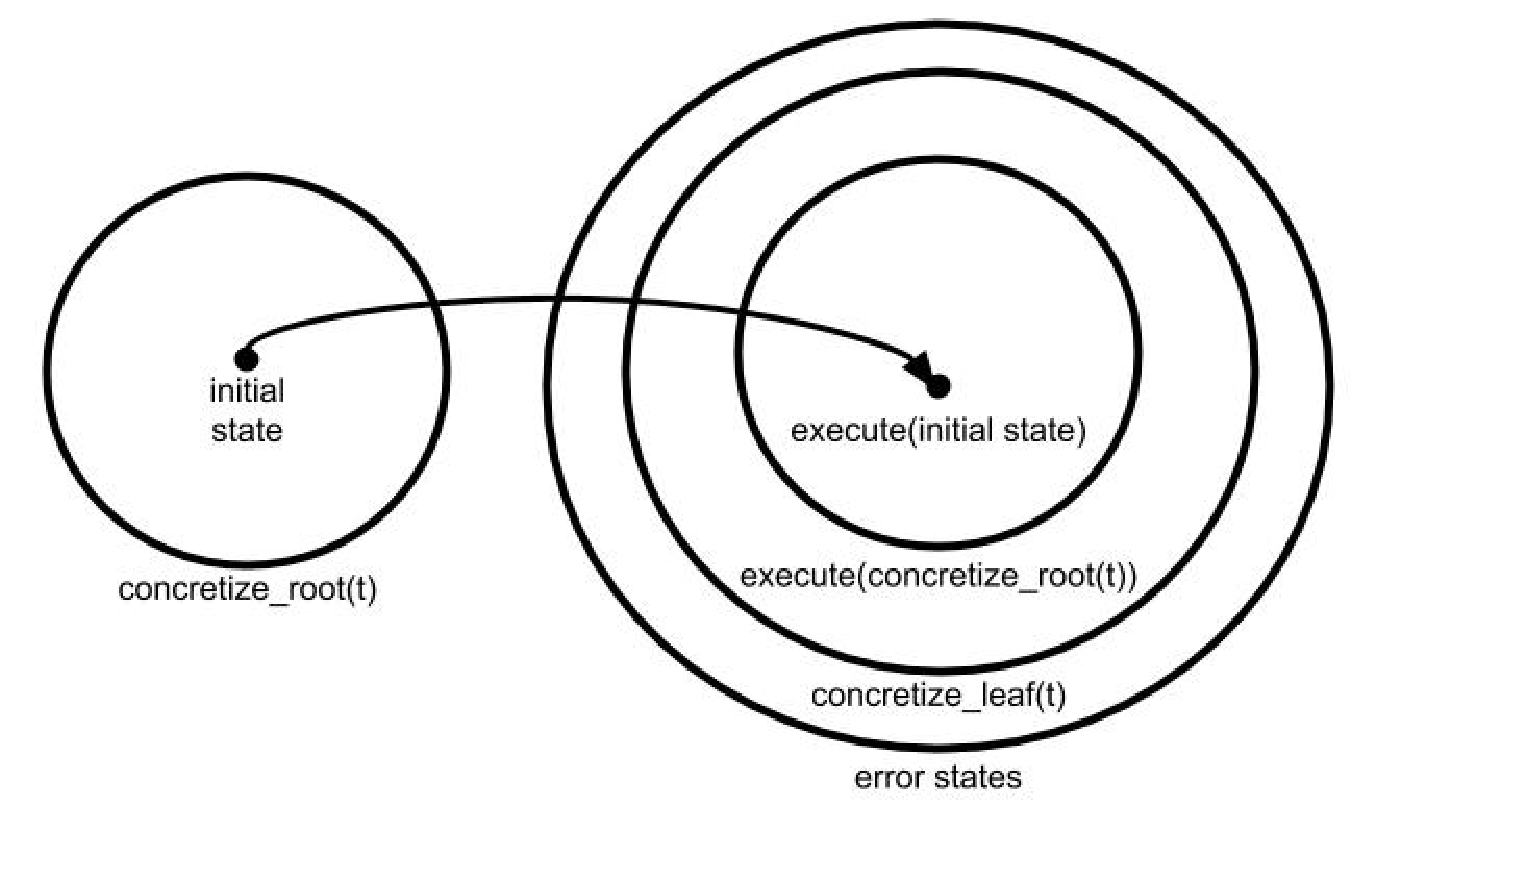
\includegraphics[width=\textwidth]{set3.eps}
\caption{Visual depiction of the base case of the proof.}
\label{fig:basecase}
\end{figure}

In other words, as depicted in Figure \ref{fig:basecase}, we show that the initial state is an element of $concretize\_root(t)$ of the tree, $t$, and that concretely executing any element of $concretize\_root(t)$ will result n an element inside $concretize\_leaf(t).$



For our inductive step, as depicted in Figures  \ref{fig:tlist} and \ref{fig:indstep}, we show that execution of each root with inputs from each specified leaf in a tree list of size $n$ will result in an element of $concretize\_leaf(t_n)$.

Our inductive hypothesis is that $execute\_tree\_list (tree\_list') \in concretize\_leaf (t_{n-1})$, where $tree\_list'$ is a $tree\_list$ with the last element removed. We then show that $concretize\_leaf (t_{n-1}) \subseteq concretize\_root (t_{n}) $, and therefore the concrete execution of any element in $concretize\_leaf (t_{n-1}) $ is in the set of of the concrete execution of any element in $concretize\_root (t_{n})$. Next, we show that $concretize\_root (t_{n}) \subseteq concretize\_leaf (t_{n})$, giving us our result.
 
\begin{figure}
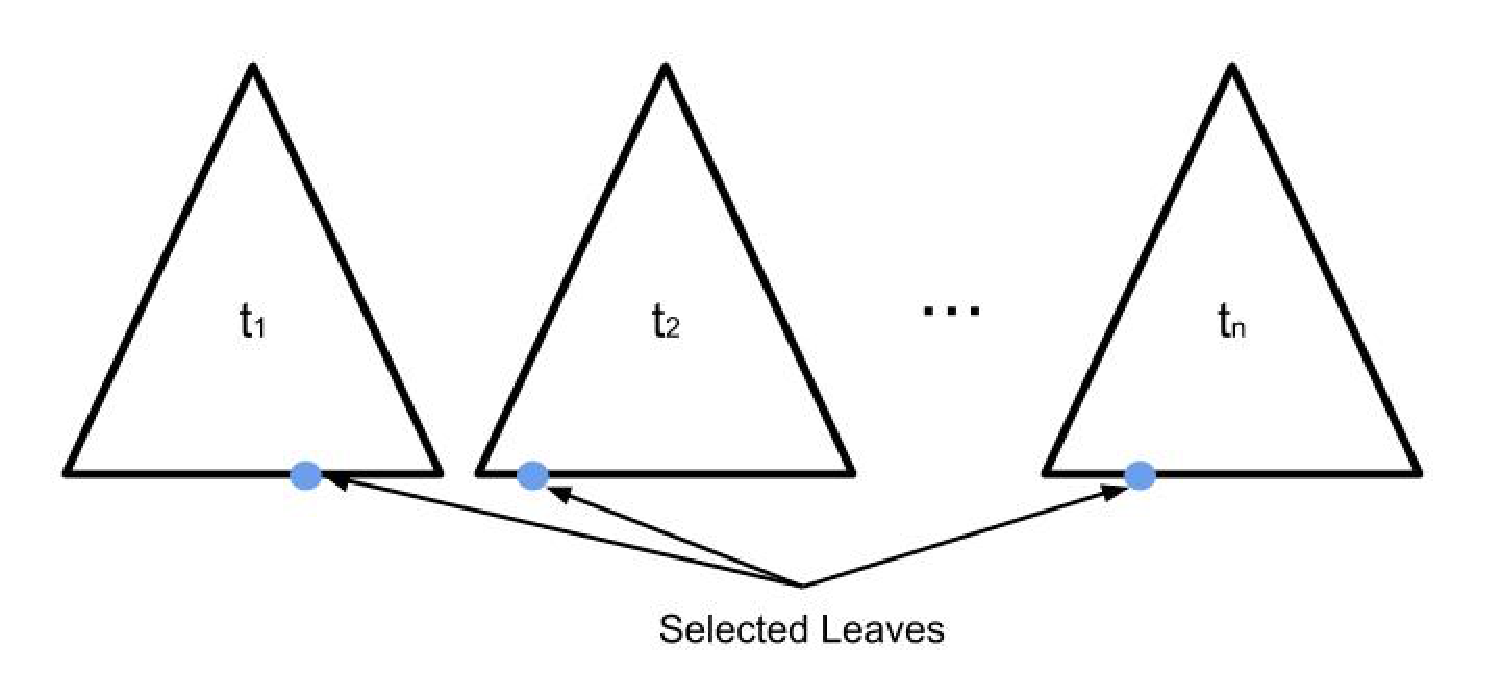
\includegraphics[width=\textwidth]{tlist.eps}
\caption{List of trees of length $n$.}
\label{fig:tlist}
\end{figure}

\begin{figure}
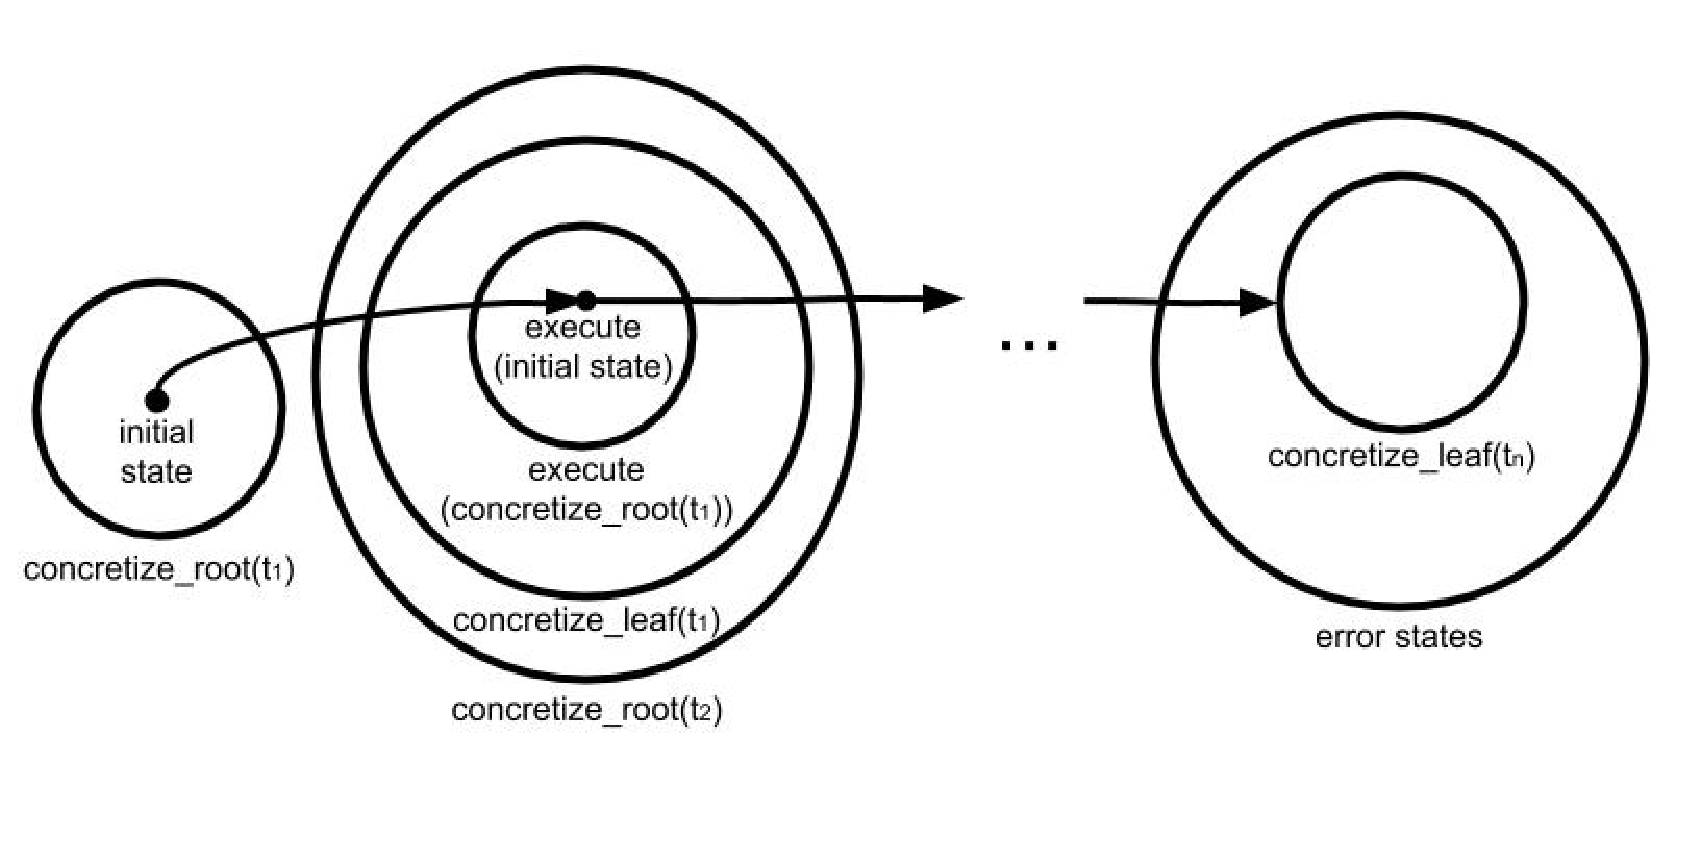
\includegraphics[width=\textwidth]{set4.eps}
\caption{Visual depiction of the inductive step of the proof.}
\label{fig:indstep}
\end{figure}

%\subsection{Formal Representation of Symbolic Execution}
In order to prove properties about symbolic execution, we created a formal, abstract representation of concrete execution and symbolic execution.
Next, we formally expressed King's property of commutativity as an axiom in order to utilize it in our tool's representation.

\subsubsection{Concrete Execution}
To represent concrete execution, we defined two abstract types: 
\begin{itemize}
\item \emph{input} represents a set of inputs into the system.
\item \emph{state\_assignments}  represents state variable assignments for the system.
\item \emph{conc\_state} represents a concrete state in the system.
\end{itemize}

\begin{define} [Concrete Execution]
$conc\_ex: \{conc\_state\} \times \{input\} \rightarrow conc\_state $.
\end{define}
To concretely execute, the \emph{conc\_ex} method takes a concrete state and an input and returns a new concrete state.


%Inductive-type Variables
%\begin{itemize}
%\item list input - list of elements of type ``input'', each element being an assignment for one input variable.
%\item list conc\_state - list of elements of type ``conc\_state'', each element being an assignment for one state variable.
%\end{itemize}

%Abstract Methods
%\begin{itemize}
%\item conc\_ex - takes a list of inputs of type ``conc\_state'' and a list of type ``input'' and outputs new list of ``conc\_state''.
%\end{itemize}


\subsubsection{Symbolic Execution}

To represent symbolic execution, we defined two abstract types:
\begin{itemize}
\item \emph{phi} is an abstract state.
\item \emph{pc} is a path constraint.
\end{itemize}

A symbolic state, or \emph{sym\_state} is a tuple of one item of type \emph{phi} and one item of type \emph{pc}.
A symbolic execution tree, or \emph{SE\_tree} is a tree structure consisting of \emph{sym\_state} elements. 


Additionally, we defined the following abstract methods:
\begin{define} [Symbolic Execution]
$sym\_ex: sym\_state \rightarrow SE\_tree $.
\end{define}

\begin{define} [PC Evaluation]
$pc\_eval: \{sym\_state\} \times \{input\} \times \{state\_assignments\} \rightarrow \{True, False\} $.
\end{define}
\emph{pc\_eval} takes the pc of a sym\_state, an input and conc\_state assignments, and returns $True$ if those assignments do not violate the path constraint.

\begin{define} [Symbolic State Instantiation]
$sym\_instantiate: \{phi(sym\_state)\} \times \{input\} \times \{state\_assignments\} \rightarrow conc\_states $.
\end{define}
 \emph{instantiate} takes the phi of a sym\_state, n input and conc\_state assignments, and instantiates them into a new list of conc\_states.
 



\subsubsection{Commutativity}
In order to assume the correctness of symbolic execution, we need to assume the following commutativity property as expressed by King (citation):
``The operation of instantiating the symbols
{$\alpha_i$} with specific integers, say {$j_i$}, and the operation of
executing the program are interchangeable. That is, if
one conventionally executes a program with a specific
$\alpha_i$'s by
$j_i$'s first, followed by execution), the results will be the
same as executing the program symbolically and then
instantiating the symbolic results (assigning $j$'s to $\alpha$'s).
The meaning of ``instantiating the symbolic results" is
first, for each terminal leaf in the execution tree, substitute
$j$'s for $\alpha$'s in all program variable values and in
pc. Then the ``results" are the values for the terminal 
node whose pc becomes true.'' (citation)


Our interpretation of this property was the following axiom:
\begin{axiom}
for all input lists $li$, conc\_state lists $lcs$, sym\_states $s$,
if there exists an SE\_tree $t$ such that
s is a leaf of t and
$pc\_eval (get_pc(s), lcs, li) = true$,
then
$conc\_ex(lcs, li) = instantiate (get\_phi (x), lcs, li)$.
\end{axiom}


\section{Formal Representation of Our Tool}
Our system contains the following three global variables:
\begin{itemize}
\item A list of SE\_trees called \textit{tree\_list} that represent the list of trees returned by our tool.
\item A list of conc\_states to represent the initial system state, or \textit{init\_conc\_state}.
\item A set of conc\_state lists to represent all of the system error states, or \textit{Error\_States}.
\end{itemize}

We then define the method \textit{execute\_tree\_list}, that takes a list of SE\_trees and executes them according to the inputs given by the leaves.

Additionally, we define the abstract method, \textit{get\_input} which returns a list of inputs that do not violate a given sym\_state's pc.
This method is bound by the requirement,
\begin{axiom}
forall SE\_trees $t$, input lists $li$, and conc\_state lists $lcs$,  
if $li = get\_input (get\_pc (l)) $, where $l$ is a leaf of $t$,
then there exists a sym\_state $s'$ such that
 $pc\_eval (get\_pc (s'), lcs, li) = True$.
\end{axiom}

\subsection{Circle Operations}
The recursive symbolic execution tool utilizes two circle operations. 
They define them in the following way: 

``Let $\mathcal{E}$ represent the symbolic exploration of one clock cycle of a processor modeled by $M$. Let $n_r = (s_r,\pi_r)$ be the root node of tree $\mathcal{E}$ and let $n_l = (s_l,\pi_l)$ be a leaf node of the same tree. 
Then $s_r \circ \pi_l$ represents the set of concrete states, and $s_l \circ \pi_l$ represents the set of concrete next-states, that are at the end-points of the path from $n_r$ to $n_l$.'' (citation)

For our proof we let $circle\_op\_1 =  s_r \circ \pi_l$ and $circle\_op\_2 =  s_l \circ \pi_l$.
Both operations take the whole SE\_tree as input.

We now can formally prove the following lemma, which we will use in our proof:
\begin{lemma} \label{cop}
forall SE\_trees $t$ and conc\_state lists $csl$,
if $csl \in circle\_op\_1(t)$,
then 
$conc\_ex(csl, get\_input (get\_pc (l))) \in circle\_op\_2(t)$,
where $l$ is a leaf of $t$.
\end{lemma}

In order to prove this, we utilize the commutativity property expressed earlier.


\subsection{Tool Requirements}
We formally express the requirements stated of the tool by Zhang et al. (citation).
The following requirements, when placed on our system, should be enough to prove that the tool works as expected:
\textbf{Axiom (Property $1$):} 
$init\_conc\_state \in circle\_op\_1 (first\_elem (tree\_list))$.

\textbf{Axiom (Property $2$):}
$ circle\_op\_2 (last\_elem (tree\_list)) \cap Error_States 
\neq empty\_set $.

\textbf{Axiom (Property $3$) :} 
for all SE\_trees $a$ $b$, 
if $a$ and $b$ are consecutive in $tree\_list$, then 
$circle\_op\_2 (a) \subseteq
circle\_op\_1 (b) $.

These properties end up not being sufficient for proving the tool works. 
We make Property 2 stronger by replacing it with the following property:

\textbf{Axiom (Property $2'$):}
$circle\_op\_2 (last\_elem (tree\_list))
\subseteq Error\_States $.



Our main sufficiency theorem that we prove is the following:
\begin{theorem}
$execute\_tree\_list (tree\_list) \in Error\_States$.
\end{theorem}
 In other words, given our three property requirements, executing our tree\_list will get us to an error state.
\section{Verification Approach}
%figures : 
We give a basic outline of our proof of our correctness theorem.

We want to show that $\mathtt{execute\_tree\_list} (tree\_list) \in error\_states$.

We prove this by first proving Theorem \ref{thm:etl}.

\begin{proof}[Theorem \ref{thm:etl}]
This is a proof by induction on the size of $tree\_list$.

For our base case we show that if $tree\_list$ is of length $1$, then $\mathtt{execute\_tree\_list} (tree\_list) \in \mathtt{concretize\_leaf} (t)$.


To prove this we use the following set property (which we verify in Coq):

\begin{theorem}
$\forall$ inputs $i$,
If $A \in B$ and 
$\forall x \in B$, \concexecution($x, i$) $\in C$, then  \concexecution($A, i$) $\in$ $C$.
\label{thm:set2}
\end{theorem}

If $tree\_list$ is of length $1$, we know we are executing from the initial concrete state of the system. Therefore, we consider the following properties:
\begin{itemize}
\item $init\_conc\_state \in 
  \mathtt{concretize\_root} (\mathtt{last\_element} (tree\_list))$. (Property $1$)
 \item $ \forall$ inputs $i$, 
 $\forall x \in
  \mathtt{concretize\_root} (\mathtt{last\_element} (tree\_list))$,  
 $ \concexecution(x, i) \in \mathtt{concretize\_leaf}(\mathtt{last\_element}(tree\_list))$.
\end{itemize}

Now, using Theorem \ref{thm:set2}, we conclude that $\concexecution(init\_conc\_state) \in \mathtt{concretize\_leaf}(\mathtt{last\_element}(tree\_list))$.

Our inductive hypothesis is  $\mathtt{execute\_tree\_list} (tree\_list') \in \mathtt{concretize\_leaf} (\mathtt{last\_element}(tree\_list'))$ where $tree\_list'$ is $tree\_list$ with the last element removed.

We want to show that if our inductive hypothesis holds, then $\mathtt{execute\_tree\_list} (tree\_list) \in \mathtt{concretize\_leaf}(tree\_list)$.

In order to prove this, we must prove the following lemma:
\begin{lemma} 
\label{lem:etl}
$\mathtt{execute\_tree\_list} (tree\_list') \in \mathtt{concretize\_root} (\mathtt{last\_element} (tree\_list))$.
\end{lemma}
\begin{proof}[Lemma \ref{lem:etl}]
We prove this using the following set property (which we verify in Coq):

\begin{theorem} \label{thm:set1}
If $A \in B$ and $B \subseteq C$, then $A \in C$.
\end{theorem}

We know:
\begin{itemize}
\item$ \mathtt{execute\_tree\_list}(tree\_list') \in
        \mathtt{concretize\_leaf} (\mathtt{last\_element}(tree\_list')) $. (Inductive Hypothesis)
\item 
$\mathtt{concretize\_leaf} (\mathtt{last\_element} tree\_list') \subseteq \mathtt{concretize\_root} (\mathtt{last\_element} tree\_list)$. (Property $3$)
 \end{itemize}
 
 So, using Theorem \ref{thm:set1}, we conclude that $\mathtt{execute\_tree\_list} (tree\_list') \in \mathtt{concretize\_root} (\mathtt{last\_element} tree\_list)$. \qed
\end{proof}

Now, to prove our inductive step, we know:
\begin{itemize}
\item $\mathtt{execute\_tree\_list} (tree\_list') \in \mathtt{concretize\_leaf} (\mathtt{last\_element}(tree\_list'))$. (Lemma \ref{lem:etl})
\item if $x \in \mathtt{concretize\_root}(\mathtt{last\_element}(tree\_list))$, then  $\concexecution(x, get\_input (l.\pathcondition)) \in \mathtt{concretize\_leaf}(\mathtt{last\_element}(tree\_list))$,
where $l$ is a leaf of $\mathtt{last\_element}(tree\_list)$. (Lemma \ref{cop})
\item $\mathtt{concretize\_leaf}(t) \neq \{\} $. (Property $3'$)
\end{itemize}

So, using Theorem \ref{thm:set2}, we can conclude that $\mathtt{execute\_tree\_list} (tree\_list) \in \mathtt{concretize\_leaf} (\mathtt{last\_element}(tree\_list))$. \qed
\end{proof}

Now, we prove our correctness property.

\begin{proof}[Theorem \ref{thm:sufficiency}]
We know:
\begin{itemize}
\item $\mathtt{execute\_tree\_list}(tree\_list) \in \mathtt{concretize\_leaf}(\mathtt{last\_element}(tree\_list))$. (Theorem \ref{thm:etl})
\item $\mathtt{concretize\_leaf} (\mathtt{last\_element} (tree\_list)) \subseteq error\_states$. (Property $2'$)
\end{itemize}
so, using Theorem \ref{thm:set1}, we conclude
$\mathtt{execute\_tree\_list} (tree\_list) \in error\_states$. \qed
\end{proof}

The reason we need Property $2'$ is because Property $2$ is not sufficient. This is because if $\mathtt{execute\_tree\_list} (tree\_list) \in \mathtt{concretize\_leaf} (\mathtt{last\_element}(tree\_list))$ and $\mathtt{concretize\_leaf} (\mathtt{last\_element} (tree\_list)) \cap error\_states \neq \{\}$, we could get the case where
$\mathtt{execute\_tree\_list} (tree\_list) \notin error\_states$, as shown in Figure \ref{fig:Prop2}.

\begin{figure}
\label{fig:Prop2}
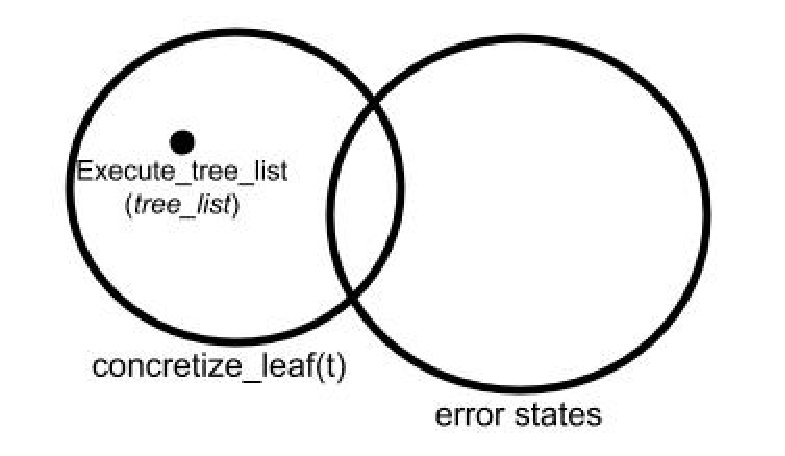
\includegraphics[width=\textwidth]{prop2.eps}
\caption{Example of Property $2$ not being sufficient to show $\mathtt{execute\_tree\_list} (tree\_list) \in error\_states$.}
\end{figure}





\section{Conclusion}

%\input scraptext
%% \input introduction
%% \input background
%% \input proofdesign
%% \input relatedwork
%% \input conclusion


\bibliographystyle{splncs04}
\bibliography{references}

\end{document}
